

A especificação HBUS define um protocolo de comunicação ponto-a-ponto. Este protocolo é explorado em detalhes neste capítulo.

\section{Estrutura de uma mensagem HBUS}

Os quadros de mensagem HBUS são constituídos de vários campos, onde se identificam os dispositivos fonte e destino da mensagem, além do conteúdo da mensagem.

\subsection{Alocação de endereços para os dispositivos}

Será usado a partir de agora o conceito de barramento local e barramento global. A especificação HBUS permite um ou mais barramento HBUS seja conectado a outro barramento por meio de um repetidor. Isto é feito para aumentar a capacidade de conexão de dispositivos no sistema como um todo. Note que ainda continuará existindo apenas um mestre. A ação da repetição do barramento gera um novo barramento com endereço diferente do originário. O barramento global é o sistema composto por todos os dispositivos HBUS conectados a todos os sub barramentos interconectados.

Cada dispositivo no barramento global possui um endereço. Este endereço é composto por dois bytes, sendo um referente ao número do barramento local no qual o dispositivo está conectado e o outro é o endereço do dispositivo dentro deste barramento.

\subsection{O pacote HBUS}

De forma geral as transmissões são realizadas em pacotes que seguem o esquema mostrado na figura a seguir. Na figura, cada quadrado representa um byte transmitido.

\newcommand{\SDSTR}{Endereço do \\ disp. fonte}
\newcommand{\TDSTR}{Endereço do \\ disp. alvo}
\newcommand{\CMDSTR}{Comando}
\newcommand{\TERMSTR}{Fim}
\newcommand{\DATASTR}{Dados}
\newcommand{\ADDRSTR}{Endereço}
\newcommand{\SIZESTR}{Tamanho}

\begin{figure}[H]
\centering
% XCircuit output "hbuspacket.tex" for LaTeX input from hbuspacket.ps
\def\putbox#1#2#3#4{\makebox[0in][l]{\makebox[#1][l]{}\raisebox{\baselineskip}[0in][0in]{\raisebox{#2}[0in][0in]{\scalebox{#3}{#4}}}}}
\def\rightbox#1{\makebox[0in][r]{#1}}
\def\centbox#1{\makebox[0in]{#1}}
\def\topbox#1{\raisebox{-0.60\baselineskip}[0in][0in]{#1}}
\def\midbox#1{\raisebox{-0.20\baselineskip}[0in][0in]{#1}}
\begin{center}
   \scalebox{1}{
   \normalsize
   \parbox{4.97917in}{
   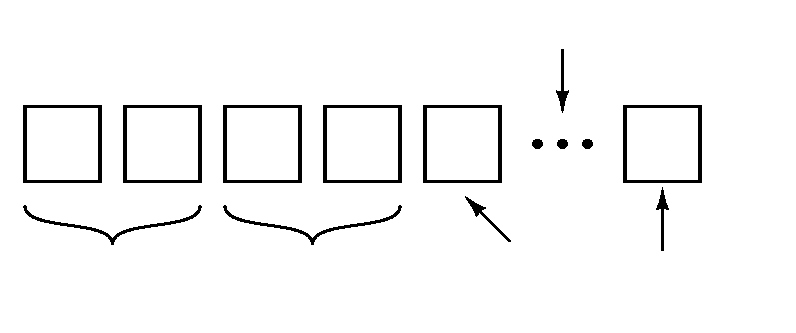
\includegraphics[scale=1]{../media/hbuspacket.ps}\\
   % translate x=448 y=354 scale 0.38
   \putbox{0.22in}{1.65in}{1.20}{0}%
   \putbox{0.89in}{1.65in}{1.20}{1}%
   \putbox{1.56in}{1.65in}{1.20}{2}%
   \putbox{2.22in}{1.65in}{1.20}{3}%
   \putbox{2.89in}{1.73in}{1.20}{}%
   \putbox{2.89in}{1.65in}{1.20}{4}%
   \putbox{4.22in}{1.65in}{1.20}{n}%
   \putbox{4.47in}{0.15in}{1.20}{\centbox{\midbox{(0xFF)}}}%
   \putbox{0.06in}{0.32in}{1.20}{Endereco do}%
   \putbox{0.14in}{0.15in}{1.20}{}%
   \putbox{0.06in}{0.15in}{1.20}{}%
   \putbox{0.06in}{0.15in}{1.20}{disp. fonte}%
   \putbox{1.47in}{0.32in}{1.20}{Endereco do}%
   \putbox{1.47in}{0.15in}{1.20}{disp. destino}%
   \putbox{2.97in}{0.32in}{1.20}{Comando}%
   \putbox{3.97in}{0.32in}{1.20}{Terminador}%
   \putbox{3.39in}{1.82in}{1.20}{Dados}%
   \putbox{3.64in}{1.90in}{1.20}{}%
   \putbox{0.31in}{1.15in}{0.96}{\centbox{\midbox{SBID}}}%
   \putbox{0.81in}{1.07in}{0.96}{\centbox{\midbox{}}}%
   \putbox{0.97in}{1.15in}{0.96}{\centbox{\midbox{SDID}}}%
   \putbox{1.64in}{1.15in}{0.96}{\centbox{\midbox{TBID}}}%
   \putbox{2.31in}{1.15in}{0.96}{\centbox{\midbox{TDID}}}%
   \putbox{2.97in}{1.15in}{0.96}{\centbox{\midbox{CMD}}}%
   \putbox{4.31in}{1.15in}{0.96}{\centbox{\midbox{STP}}}%
   } % close 'parbox'
   } % close 'scalebox'
   \vspace{-\baselineskip} % this is not necessary, but looks better
\end{center}

%\import{../media/}{hbuspacket}
\caption{Pacote HBUS}
\end{figure}

Dependendo do comando, a seção de dados do pacote pode conter um número diferente de bytes. Para alguns comandos este número pode ser inclusive zero.

O byte terminador tem valor obrigatório de 0xFF.

\section{Os comandos HBUS}

O conjunto de comandos padrão do barramento HBUS é discutido. A tabela mostra a lista de comando disponíveis.

\begin{table}[H]
\centering
\caption{Comandos HBUS}
\begin{tabular}{c c p{4cm} p{6cm}}
\hline
Comando	 &	 Código 		&	Parâmetros				&	 Descrição\\
\hline
SETCH	&	0x01			&	Endereço	 do objeto e tamanho em bytes		&	Escreve no objeto do dispositivo se o mesmo tem permissão de escrita\\
GETCH	&	0x04			&	Endereço do objeto		&	Lê objeto do dispositivo caso tenha permissão de leitura\\
RESPONSE&	0x10			&	Endereço do objeto origem e tamanho em bytes & Envia o valor do objeto que foi requisitado pelo comando GETCH\\
SEARCH	&	0x03			&	---						&	Inicia o processo de endereçamento dos dispositivos ou verifica presença de um dispositivo já endereçado\\
ACK		&	0x06			&	---						&	Comando para indicar que mestre ou dispositivo confirmaram algum processo anterior.\\
ERROR	&	0x20			&	Código de erro			&	Comando para retorno de códigos de erro. Opcional.\\
QUERY	&	0x07		&	Endereço do objeto		&	Lê informações sobre o objeto. O dispositivo envia a estrutura HBUSOBJINFO.\\
QUERY\_EP &	0x11		&	Endereço do endpoint		&	Análogo ao comando QUERY, porém voltado aos endpoints.\\
QUERY\_INT&	0x12		&	Endereço da interrupção	&	Funcionamento similar aos dois comandos anteriores.\\
QUERY\_RESP & 0x08		&	Endereço do objeto origem & As informações do objeto, endpoints e interrupções são retornadas através deste comando.\\
STREAMW	&	0x40			&	Endereço do endpoint e tamanho do bloco		&	Realiza escrita no endpoint selecionado se houver permissão.\\
STREAMR	&	0x41			&	Endereço do endpoint		&	Realiza leitura no endpoint.\\
BUSLOCK	&	0xF0			&	---						& 	Causa o travamento exclusivo do barramento para comunicações entre os dois dispositivos envolvidos na mensagem.\\
BUSUNLOCK&	0xF1			&	---						&	Finaliza o travamento exclusivo do barramento, liberando-o.\\
SOFTRESET&	0xF2			&	---						&	Ocasiona um RESET por software no dispositivo.\\
KEYSET	&	0xA0			&	Chave pública do mestre	&	Registra chave pública do mestre no dispositivo.\\
KEYRESET	&	0xA1			&	Bloco de assinatura		&	Remove registro de chave pública do dispositivo.\\
\hline
\end{tabular}
\end{table}

A seguir uma análise mais detalhada é feita.

\subsection{Os comandos SETCH, GETCH e RESPONSE}

Esses três comandos estão envolvidos com a tarefa de escrita e leitura em objetos do dispositivo.

\subsubsection{SETCH}

O comando \hbuscommand{SETCH} realiza a escrita em um objeto do dispositivo. O dispositivo deve, após aceitar o comando, verificar se o objeto possui permissão de escrita. Caso possua, o novo valor enviado é escrito no objeto. Caso contrário o dispositivo pode enviar de volta uma mensagem utilizando o comando \hbuscommand{ERROR} ou não enviar nada.

Os parâmetros do comando \hbuscommand{SETCH} são o endereço do objeto no dispositivo e o tamanho em bytes a ser escrito. A figura \ref{fig:setch} mostra a estrutura de uma mensagem usando o comando \hbuscommand{SETCH}. Não é mostrada a parte inicial de endereçamento para simplicidade.

\begin{figure}[H]
\centering
% XCircuit output "setch.tex" for LaTeX input from setch.ps
\def\putbox#1#2#3#4{\makebox[0in][l]{\makebox[#1][l]{}\raisebox{\baselineskip}[0in][0in]{\raisebox{#2}[0in][0in]{\scalebox{#3}{#4}}}}}
\def\rightbox#1{\makebox[0in][r]{#1}}
\def\centbox#1{\makebox[0in]{#1}}
\def\topbox#1{\raisebox{-0.60\baselineskip}[0in][0in]{#1}}
\def\midbox#1{\raisebox{-0.20\baselineskip}[0in][0in]{#1}}
\begin{center}
   \scalebox{1}{
   \normalsize
   \parbox{4.08333in}{
   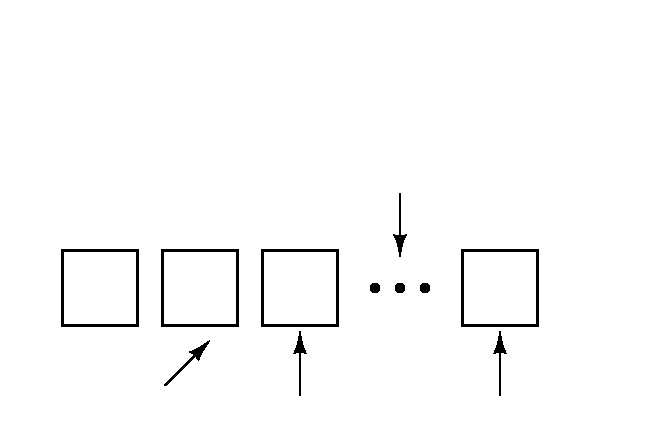
\includegraphics[scale=1,trim= 0 0 0 1.5cm]{setch.ps}\\
   % translate x=544 y=352 scale 0.38
   \putbox{3.39in}{1.72in}{1.20}{}%
   \putbox{0.47in}{1.39in}{1.20}{4}%
   \putbox{3.14in}{1.39in}{1.20}{n}%
   \putbox{3.22in}{0.89in}{1.20}{\centbox{\midbox{0xFF}}}%
   \putbox{0.64in}{0.14in}{1.20}{}%
   \putbox{0.56in}{0.14in}{1.20}{}%
   \putbox{2.89in}{0.06in}{1.20}{Terminador}%
   \putbox{2.31in}{1.56in}{1.20}{Dados}%
   \putbox{4.14in}{1.89in}{1.20}{}%
   \putbox{0.56in}{0.89in}{1.20}{\centbox{\midbox{0x01}}}%
   \putbox{1.14in}{1.39in}{1.20}{5}%
   \putbox{0.39in}{0.06in}{1.20}{Endereco}%
   \putbox{1.81in}{1.39in}{1.20}{6}%
   \putbox{1.56in}{0.06in}{1.20}{Tamanho}%
   \putbox{1.22in}{0.89in}{0.96}{\centbox{\midbox{ADDR}}}%
   \putbox{1.89in}{0.89in}{0.96}{\centbox{\midbox{PSZ}}}%
   \putbox{2.56in}{0.72in}{0.96}{\centbox{\midbox{PRM}}}%
   } % close 'parbox'
   } % close 'scalebox'
   \vspace{-\baselineskip} % this is not necessary, but looks better
\end{center}

\caption{O comando \hbuscommand{SETCH}}
\label{fig:setch}
\end{figure}

\subsubsection{GETCH}

Este comando realiza a leitura de um objeto do dispositivo. Após aceitar o comando, se o objeto tem permissão de leitura, o dispo sito enviará um comando \hbuscommand{RESPONSE} contendo os dados do objeto. Caso contrário pode enviar ou não uma mensagem com o comando \hbuscommand{ERROR}.

\begin{figure}[H]
\centering
\documentclass[border=10pt]{standalone}
\usepackage{tikz}

\usetikzlibrary{positioning,arrows,decorations.pathreplacing}

\begin{document}

%Provide default strings for packet field descriptions in english if anything else not set

\providecommand{\ADDRSTR}{Address}
%\providecommand{\SIZESTR}{Size}
\providecommand{\TERMSTR}{Terminator}
%\providecommand{\DATASTR}{Data}
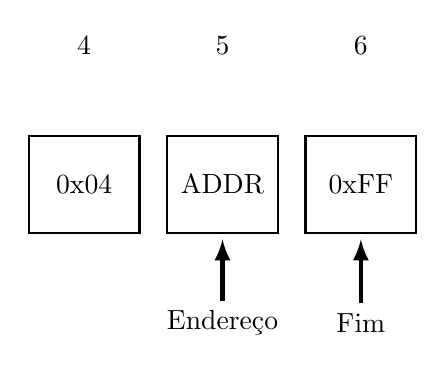
\begin{tikzpicture}[node distance=50pt,minimum size=1pt,auto]

\tikzstyle{pfield}=[rectangle,minimum width=40pt,minimum height=35pt,draw=black,thick];

\node [pfield] (b0) {0x04};
\node [pfield] (b1) [right of=b0] {ADDR};
%\node [pfield] (b2) [right of=b1] {PSZ};
%\node [pfield] (b3) [right of=b2] {ADDR};
%\node [pfield] (b4) [right of=b3] {PSZ};

%\node  (d0) [right of=b2,xshift=-10pt] {$\bullet$};
%\node  (d1) [right of=d0,xshift=-35pt] {$\bullet$};
%\node  (d2) [right of=d1,xshift=-35pt] {$\bullet$};

\node [pfield] (b5) [right of=b1] {0xFF};

%\draw [decorate,decoration={brace,amplitude=10pt,raise=5pt}] (b1.315) -- (b0.225) node [black,midway,align=center,yshift=-15pt] {\SDSTR};

%\draw [decorate,decoration={brace,amplitude=10pt,raise=5pt}] (b3.315) -- (b2.225) node (t0) [black,midway,align=center,yshift=-15pt] {\TDSTR};

%\node (t1) at (t0 -| b4) {\CMDSTR};

%\node (t1) [above of=d1] {\DATASTR};
\node (t2) [below of=b1] {\ADDRSTR};
%\node (t3) at (t2 -| b2) {\SIZESTR};

\node [align=center] (t4) at (t2 -| b5) {\TERMSTR};

%\path [-latex,ultra thick, shorten >=5pt] (t1) edge (d1);
\path [-latex,ultra thick, shorten >=2pt] (t4) edge (b5);
%\path [-latex,ultra thick, shorten >=2pt] (t3) edge (b2);
\path [-latex,ultra thick, shorten >=2pt] (t2) edge (b1);

%field number
\node [above of=b0] {4};
\node [above of=b1] {5};
%\node [above of=b2] {6};
%\node [above of=b3] {N};
%\node [above of=b4] {6};
\node [above of=b5] {6};

\end{tikzpicture}
\end{document}
\caption{O comando \hbuscommand{GETCH}}
\end{figure}

\subsubsection{RESPONSE}

Após a utilização do comando \hbuscommand{GETCH}, o dispositivo deve retornar a informação através do comando \hbuscommand{RESPONSE}.
A estrutura parcial da mensagem é vista a seguir.

\begin{figure}[H]
\centering
\documentclass[border=10pt]{standalone}
\usepackage{tikz}

\usetikzlibrary{positioning,arrows,decorations.pathreplacing}

\begin{document}

%Provide default strings for packet field descriptions in english if anything else not set

\providecommand{\ADDRSTR}{Address}
\providecommand{\SIZESTR}{Size}
\providecommand{\TERMSTR}{Terminator}
\providecommand{\DATASTR}{Data}

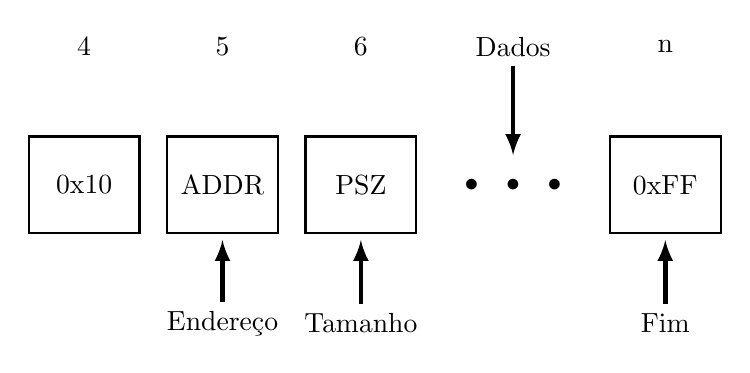
\begin{tikzpicture}[node distance=50pt,minimum size=1pt,auto]

\tikzstyle{pfield}=[rectangle,minimum width=40pt,minimum height=35pt,draw=black,thick];

\node [pfield] (b0) {0x10};
\node [pfield] (b1) [right of=b0] {ADDR};
\node [pfield] (b2) [right of=b1] {PSZ};
%\node [pfield] (b3) [right of=b2] {ADDR};
%\node [pfield] (b4) [right of=b3] {PSZ};

\node  (d0) [right of=b2,xshift=-10pt] {$\bullet$};
\node  (d1) [right of=d0,xshift=-35pt] {$\bullet$};
\node  (d2) [right of=d1,xshift=-35pt] {$\bullet$};

\node [pfield] (b5) [right of=d2,xshift=-10pt] {0xFF};

%\draw [decorate,decoration={brace,amplitude=10pt,raise=5pt}] (b1.315) -- (b0.225) node [black,midway,align=center,yshift=-15pt] {\SDSTR};

%\draw [decorate,decoration={brace,amplitude=10pt,raise=5pt}] (b3.315) -- (b2.225) node (t0) [black,midway,align=center,yshift=-15pt] {\TDSTR};

%\node (t1) at (t0 -| b4) {\CMDSTR};

\node (t1) [above of=d1] {\DATASTR};
\node (t2) [below of=b1] {\ADDRSTR};
\node (t3) at (t2 -| b2) {\SIZESTR};

\node [align=center] (t4) at (t2 -| b5) {\TERMSTR};

\path [-latex,ultra thick, shorten >=5pt] (t1) edge (d1);
\path [-latex,ultra thick, shorten >=2pt] (t4) edge (b5);
\path [-latex,ultra thick, shorten >=2pt] (t3) edge (b2);
\path [-latex,ultra thick, shorten >=2pt] (t2) edge (b1);

%field number
\node [above of=b0] {4};
\node [above of=b1] {5};
\node [above of=b2] {6};
%\node [above of=b3] {N};
%\node [above of=b4] {6};
\node [above of=b5] {n};

\end{tikzpicture}
\end{document}
\caption{O comando \hbuscommand{RESPONSE}}
\end{figure}

\subsection{Os comandos QUERY, QUERY\_EP, QUERY\_INT e QUERY\_RESP}

Estes comandos são relacionados a obtenção de informações sobre os objetos de dispositivo e suas variações: endpoints e interrupções. O mestre não precisa ter conhecimento prévio sobre um dispositivo qualquer que é conectado ao barramento. Através deste mecanismo, ele pode obter todas as informações através do próprio barramento.

Os comandos \hbuscommand{QUERY}, \hbuscommand{QUERY\_EP} e \hbuscommand{QUERY\_INT} buscam informações dos objetos de dispositivo, endpoints e interrupções, respectivamente.

\begin{figure}[H]
\centering
% XCircuit output "query.tex" for LaTeX input from query.ps
\def\putbox#1#2#3#4{\makebox[0in][l]{\makebox[#1][l]{}\raisebox{\baselineskip}[0in][0in]{\raisebox{#2}[0in][0in]{\scalebox{#3}{#4}}}}}
\def\rightbox#1{\makebox[0in][r]{#1}}
\def\centbox#1{\makebox[0in]{#1}}
\def\topbox#1{\raisebox{-0.60\baselineskip}[0in][0in]{#1}}
\def\midbox#1{\raisebox{-0.20\baselineskip}[0in][0in]{#1}}
\begin{center}
   \scalebox{1}{
   \normalsize
   \parbox{4.08333in}{
   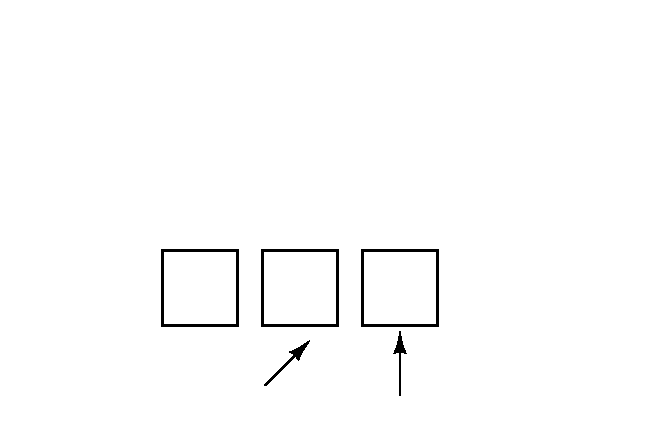
\includegraphics[scale=1,trim=0 0 0 1.5cm]{../media/query.ps}\\
   % translate x=544 y=352 scale 0.38
   \putbox{3.39in}{1.72in}{1.20}{}%
   \putbox{1.14in}{1.39in}{1.20}{4}%
   \putbox{2.47in}{1.39in}{1.20}{6}%
   \putbox{2.56in}{0.89in}{1.20}{\centbox{\midbox{0xFF}}}%
   \putbox{0.64in}{0.14in}{1.20}{}%
   \putbox{0.56in}{0.14in}{1.20}{}%
   \putbox{2.22in}{0.06in}{1.20}{Terminador}%
   \putbox{4.14in}{1.89in}{1.20}{}%
   \putbox{1.22in}{1.06in}{0.96}{\centbox{\midbox{0x07}}}%
   \putbox{1.81in}{1.39in}{1.20}{5}%
   \putbox{1.06in}{0.06in}{1.20}{Endereço}%
   \putbox{1.22in}{0.89in}{0.96}{\centbox{\midbox{0x11}}}%
   \putbox{1.22in}{0.72in}{0.96}{\centbox{\midbox{0x12}}}%
   } % close 'parbox'
   } % close 'scalebox'
   \vspace{-\baselineskip} % this is not necessary, but looks better
\end{center}

\caption{Os comandos \hbuscommand{QUERY}}
\end{figure}

O comando \hbuscommand{QUERY\_RESP} é enviado pelo dispositivo em resposta a recepção de um comando tipo \hbuscommand{QUERY($\cdots$)}. Junto a este comando é enviada a estrutura do tipo \textbf{HBUSOBJINFO}, \textbf{HBUSEPINFO} ou \textbf{HBUSINTINFO} correspondente ao objeto no dispositivo.

\begin{figure}[H]
\centering
\documentclass[border=10pt]{standalone}
\usepackage{tikz}

%Provide default strings for packet field descriptions in english if anything else not set

\providecommand{\ADDRSTR}{Address}
\providecommand{\SIZESTR}{Size}
\providecommand{\TERMSTR}{Terminator}
\providecommand{\DATASTR}{Data}

\usetikzlibrary{positioning,arrows,decorations.pathreplacing}

\begin{document}
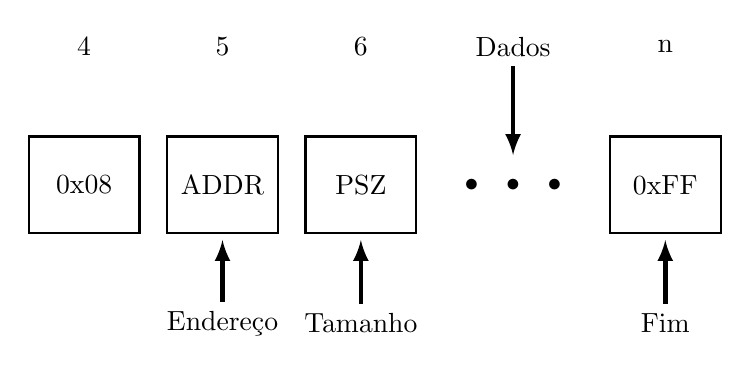
\begin{tikzpicture}[node distance=50pt,minimum size=1pt,auto]

\tikzstyle{pfield}=[rectangle,minimum width=40pt,minimum height=35pt,draw=black,thick];

\node [pfield] (b0) {0x08};
\node [pfield] (b1) [right of=b0] {ADDR};
\node [pfield] (b2) [right of=b1] {PSZ};
%\node [pfield] (b3) [right of=b2] {ADDR};
%\node [pfield] (b4) [right of=b3] {PSZ};

\node  (d0) [right of=b2,xshift=-10pt] {$\bullet$};
\node  (d1) [right of=d0,xshift=-35pt] {$\bullet$};
\node  (d2) [right of=d1,xshift=-35pt] {$\bullet$};

\node [pfield] (b5) [right of=d2,xshift=-10pt] {0xFF};

%\draw [decorate,decoration={brace,amplitude=10pt,raise=5pt}] (b1.315) -- (b0.225) node [black,midway,align=center,yshift=-15pt] {\SDSTR};

%\draw [decorate,decoration={brace,amplitude=10pt,raise=5pt}] (b3.315) -- (b2.225) node (t0) [black,midway,align=center,yshift=-15pt] {\TDSTR};

%\node (t1) at (t0 -| b4) {\CMDSTR};

\node (t1) [above of=d1] {\DATASTR};
\node (t2) [below of=b1] {\ADDRSTR};
\node (t3) at (t2 -| b2) {\SIZESTR};

\node [align=center] (t4) at (t2 -| b5) {\TERMSTR};

\path [-latex,ultra thick, shorten >=5pt] (t1) edge (d1);
\path [-latex,ultra thick, shorten >=2pt] (t4) edge (b5);
\path [-latex,ultra thick, shorten >=2pt] (t3) edge (b2);
\path [-latex,ultra thick, shorten >=2pt] (t2) edge (b1);

%field number
\node [above of=b0] {4};
\node [above of=b1] {5};
\node [above of=b2] {6};
%\node [above of=b3] {N};
%\node [above of=b4] {6};
\node [above of=b5] {n};

\end{tikzpicture}
\end{document}
\caption{O comando \hbuscommand{QUERY\_RESP}}
\end{figure}

\subsection{Os comandos STREAMW e STREAMR}

Estes comandos tem como finalidade o início de escrita e leitura de um bloco de bytes em um dos endpoints do dispositivo. Seu funcionamento é descrito a seguir.

\subsection{Os comandos BUSLOCK e BUSUNLOCK}

Utilizados como peça chave em algumas operações do barramento, além de poderem ser usados livremente pelo mestre, esses comandos tem como finalidade o travamento exclusivo do barramento para tráfego de dados entre dois dispositivos.

Todos os dispositivos escutam o barramento constantemente. Ao detectar a emissão de um comando \hbuscommand{BUSLOCK} no barramento, o dispositivo deve verificar se aquele comando é endereçado a ele. Caso seja, ele aceitará as transmissões posteriores. Caso contrário, deve ignorar todas as transmissões até que seja emitido no barramento o comando \hbuscommand{BUSUNLOCK}.

É uma definição obrigatória que o período máximo de duração de um \hbuscommand{BUSLOCK} é de 1 minuto. Se esse tempo for atingido sem a emissão de um comando \hbuscommand{BUSUNLOCK}, os dispositivos devem automaticamente sair do estado travado e aceitar transmissões.

\subsection{O comando SEARCH}

O comando \hbuscommand{SEARCH} é utilizado para duas finalidades diferentes:

\begin{enumerate}

\item Utilizado no processo de endereçamento dos dispositivos;
\item Utilizado para monitorar a presença de um dispositivo já endereçado no barramento. Este procedimento é simples e tem dois passos:
\begin{enumerate}
\item O mestre envia o comando \hbuscommand{SEARCH}.
\item O dispositivo, se ainda está presente no barramento, é obrigado a enviar o comando \hbuscommand{ACK}.
\item O mestre aguarda. Se receber o comando \hbuscommand{ACK}, sabe que o dispositivo está ativo. Se se passar um tempo especificado e não for recebido o comando, sabe-se que o dispositivo se desconectou do barramento.
\end{enumerate}

\end{enumerate}

\subsubsection{Recomendação de implementação}

É recomendado que o mestre monitore o barramento com uma frequência dependente da natureza da rede implantada utilizando-se do barramento HBUS. Na grande maioria das vezes a rede é fixa e não sofre mudanças, de forma que geralmente esse monitoramento ocorrerá em um período relaxado.

As principais razões para realizar o monitoramento periódico da rede com o comando \hbuscommand{SEARCH} são óbvias:
detecção de novos dispositivos e detecção da desconexão (ou falha) de dispositivos.

\subsection{Os comandos ACK e ERROR}

Os comandos \hbuscommand{ACK} e \hbuscommand{ERROR} servem para enviar respostas positivas e negativas, respectivamente, ao mestre. São usados em situações específicas descritas neste documento.

\subsection{O comando INT}

O comando \hbuscommand{INT} é enviado pelo dispositivo no processo de interrupção. Este processo é discutido num capítulo próximo.

\subsection{O comando SOFTRESET}

Este comando, quando recebido pelo dispositivo, requer que o mesmo execute um reset por software nele mesmo.
Na plataforma utilizada para o desenvolvimento, isto é alcançado realizando-se a execução proposital de uma instrução ilegal.

\subsection{Os comandos KEYSET E KEYRESET}

Presentes a partir da versão 1.1, estes comandos são reconhecidos apenas por dispositivos que possuem suporte a autenticação de mestre.

\subsubsection{KEYSET}

O comando \hbuscommand{KEYSET} é executado no processo de endereçamento apenas no caso de o dispositivo em questão suportar a autenticação de mestre. Através deste comando é informada ao dispositivo a chave pública do mestre, utilizada para assinar as mensagens de escrita e garantir a autenticidade das mesmas.

Este comando somente grava uma nova chave no dispositivo caso o mesmo não tenha sido previamente associado a nenhum mestre. Neste caso, ao receber o comando, o dispositivo automaticamente grava de forma permanente a chave e torna-se associado ao mestre que enviou o comando. A única maneira de o dispositivo ser desassociado deste mestre é a emissão de um comando \hbuscommand{KEYRESET}, assinado corretamente.

Caso o dispositivo já esteja associado a um mestre e receber o comando \hbuscommand{KEYSET} no processo de endereçamento, o dispositivo compara a chave recebida com a sua chave previamente gravada e duas situações são possíveis:

\begin{enumerate}

\item As chaves são iguais e o dispositivo está sendo endereçado pelo mestre correto. O dispositivo entra em operação normal.

\item As chaves são diferentes e o dispositivo está sendo endereçado por um outro mestre. Neste caso o dispositivo tem a escolha de recusar o endereçamento ou entrar em modo de operação somente leitura.

\end{enumerate}

\subsubsection{KEYRESET}

Este comando realiza a desassociação do dispositivo com o mestre. É necessário que este comando contenha uma assinatura válida.

Esta ação libera o dispositivo para ser utilizado em outros barramentos, com outro mestre.

\section{O processo de endereçamento do dispositivo}

Todos os dispositivos, quando conectados ao barramento, necessitam esperar que o mestre realize o processo de endereçamento. Mais uma vez é seguida a filosofia de não-ocupação do canal.

O dispositivo, na sua inicialização assume o endereço 255 no barramento. Este é um endereço especial reservado.

\subsection{O endereço de broadcast}

O endereço reservado 255 é chamado de endereço de broadcast, porque todos os dispositivos ainda não-endereçados são obrigados a escutar o barramento neste endereço e obedecer quaisquer mensagens que sejam direcionadas ao endereço de broadcast.

É através deste endereço, que é iniciado o processo de endereçamento do dispositivo.

\subsection{Endereçamento passo a passo}

Uma descrição passo a passo do processo de endereçamento do dispositivo:

\begin{enumerate}

\item O dispositivo completa sua inicialização e aguarda, escutando o barramento no endereço 255.
\item O mestre dá início ao processo de endereçamento através do envio de um comando \textbf{SEARCH} para o endereço de broadcast.
\item O dispositivo aguarda um período de guarda de alguns milissegundos que é definido aleatoriamente. A razão para isto é discutida em seguida.
\item Após passado o período de guarda, o dispositivo envia um comando \hbuscommand{BUSLOCK} para o mestre. O barramento está então travado. O dispositivo aguarda o mestre.
\item O mestre deve enviar um comando \hbuscommand{GETCH}, requisitando o objeto 0 do dispositivo, para obter suas funcionalidades.
\item O dispositivo envia o conteúdo do objeto 0 ao mestre.
\item Se o dispositivo tem suporte a autenticação, o mestre envia o comando \hbuscommand{KEYSET}, acompanhado da sua chave pública, endereçado ao endereço que será atribuído.
\item Caso o dispositivo não possua suporte a autenticação, o mestre envia novamente o comando \hbuscommand{SEARCH}, porém desta vez para o endereço que será atribuído ao dispositivo.
\item O dispositivo recebe o comando e assume o endereço contido no pacote.
\item O dispositivo envia o comando \hbuscommand{BUSUNLOCK} e o barramento é destravado. Chega ao fim o processo de endereçamento.

\end{enumerate}

\subsection{Prevenção de colisões no endereçamento}

Quando um barramento desenergizado com vários dispositivos já conectados é alimentado, todos os dispositivos estão no estado não-endereçado. Quando o mestre emitir o comando \hbuscommand{SEARCH}, é preciso que haja algum esquema para impedir a colisão de dispositivos que tem inicialmente o mesmo endereço (broadcast) ao tentar realizar o endereçamento.

Para isso é estabelecido o período de guarda aleatório mencionado anteriormente. Sendo o período aleatório, fatalmente um dispositivo irá travar o barramento antes dos demais, garantindo que só ele está realizando o processo de endereçamento nesta etapa, uma vez que os outros dispositivos, sabendo do estado ocupado do barramento não podem tentar realizar transmissões.

Quando o barramento estiver livre novamente, os outros dispositivos podem iniciar seu processo de endereçamento, aplicando sempre o período de guarda aleatório. Dessa maneira, os dispositivos vão completando o processo de endereçamento sucessivamente até que todos estejam endereçados no barramento.

\subsection{Recomendações}

É recomendado que assim que o processo de endereçamento for terminado, o mestre realize a identificação dos objetos através dos comandos \hbuscommand{QUERY}, obtendo assim informações sobre todos os objetos de todos os dispositivos conectados. Essas informações devem ser guardadas para facilitar o acesso aos dispositivos durante a execução.

\section{O acesso aos objetos do tipo endpoint}

O acesso a estes objetos é feito através dos comandos \hbuscommand{STREAMW} e \hbuscommand{STREAMR}. No entanto, estes comandos apenas iniciam o processo de acesso, que é feito em algumas etapas:

\begin{enumerate}

\item O mestre envia um comando \hbuscommand{STREAMW} ou \hbuscommand{STREAMR} ao dispositivo.
\item O dispositivo recebe o comando e se as permissões do endpoints forem coerentes com o comando recebido, o dispositivo executa um comando \hbuscommand{BUSLOCK}, travando o uso do barramento entre ele e o mestre.
\item No ato da recepção do \textbf{BUSLOCK}, o mestre assume que a transmissão será realizada. No caso de uma transmissão de escrita, o mestre envia os dados ao barramento travado, não sendo nenhum tipo de formatação requerida.
No caso de uma transmissão de leitura, o escravo, após executar o \hbuscommand{BUSLOCK}, começa a enviar imediatamente os dados.
\item Após a transmissão ser concluída, o escravo emite o comando \hbuscommand{BUSUNLOCK}, liberando o barramento para as comunicações.

\end{enumerate}

\subsection{A importância e expansibilidade dos endpoints}

Pode não ser aparente a primeira vista, porém o sistema de endpoints tem uma importância chave.

Devido a natureza da transmissão, que é realizada sobre o barramento travado exclusivamente para os dois dispositivos envolvidos e ainda o detalhe que durante a transmissão, os dispositivos não processam os dados da forma usual mostrada até agora, deixa-se aberta a possibilidade de implementação de protocolo secundários sobre o protocolo de comunicação HBUS através do uso de endpoints.

Esses protocolos secundários podem ser muito importantes para o dispositivo específico e variar desde sistemas para correção de erros até protocolos de comunicação complexos e desconhecidos ao barramento HBUS.

\section{Interrupções}

O sistema de interrupções tem um capítulo dedicado exclusivamente a sua discussão.

\section{O conjunto de  máquinas de estados de comunicação HBUS}

O protocolo de comunicação no dispositivo é implementado por uma máquina de estados que recebe byte a byte a transmissão e dependendo dos valores detectados, seleciona a ação apropriada.

O comportamento é como descrito até agora, observando cada tipo de comando enviado ao dispositivo. A máquina de estados também gerencia o endereçamento e eventos de travamento do barramento, além de timeouts que ocorrem se a comunicação for abandonada em meio a um pacote. Isto é necessário para garantir que o barramento não seja travado por um dispositivo operando erroneamente.

\subsection{A função SERIAL\_IDLE()}

A função SERIAL\_IDLE() verifica se está ocorrendo alguma transmissão no barramento e retorna um valor informando a situação atual. É necessário utilizar esta função todas as vezes que o dispositivo transmite alguma informação no barramento, uma vez que o canal de comunicação é half-duplex.

\subsection{A função SERIAL\_CYCLE()}

Esta é a função executada ciclicamente. Ela verifica o estado do barramento para decidir o momento de realização de transmissões e também gerencia os timeouts de comunicação.

\begin{figure}[H]
\centering
% XCircuit output "serialcycle.tex" for LaTeX input from serialcycle.ps
\def\putbox#1#2#3#4{\makebox[0in][l]{\makebox[#1][l]{}\raisebox{\baselineskip}[0in][0in]{\raisebox{#2}[0in][0in]{\scalebox{#3}{#4}}}}}
\def\rightbox#1{\makebox[0in][r]{#1}}
\def\centbox#1{\makebox[0in]{#1}}
\def\topbox#1{\raisebox{-0.60\baselineskip}[0in][0in]{#1}}
\def\midbox#1{\raisebox{-0.20\baselineskip}[0in][0in]{#1}}
\begin{center}
   \scalebox{0.6}{
   \normalsize
   \parbox{4.02083in}{
   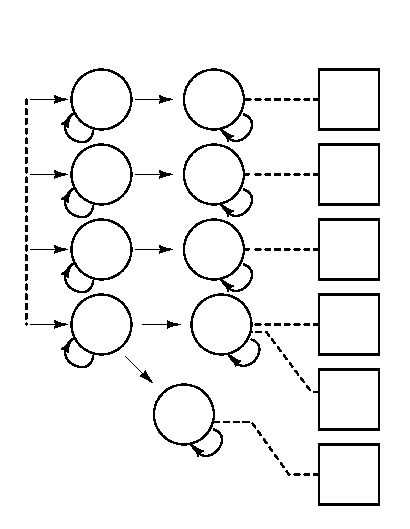
\includegraphics[scale=1.66667]{../media/serialcycle.ps}\\
   % translate x=643 y=991 scale 0.23
   \putbox{0.94in}{4.67in}{0.72}{\centbox{\midbox{SERIAL}}}%
   \putbox{0.94in}{4.50in}{0.72}{\centbox{\midbox{IDLE?}}}%
   \putbox{1.44in}{4.67in}{0.72}{\centbox{\midbox{S}}}%
   \putbox{2.11in}{4.67in}{0.72}{\centbox{\midbox{TX}}}%
   \putbox{2.19in}{4.50in}{0.72}{\centbox{\midbox{PEND?}}}%
   \putbox{3.69in}{4.67in}{0.72}{\centbox{\midbox{PROCESS}}}%
   \putbox{3.61in}{4.50in}{0.72}{\centbox{\midbox{TX}}}%
   \putbox{2.86in}{4.67in}{0.72}{\centbox{\midbox{S}}}%
   \putbox{0.86in}{3.84in}{0.72}{\centbox{\midbox{RX}}}%
   \putbox{0.94in}{3.67in}{0.72}{\centbox{\midbox{SBID?}}}%
   \putbox{2.19in}{3.84in}{0.72}{\centbox{\midbox{TIME}}}%
   \putbox{2.19in}{3.67in}{0.72}{\centbox{\midbox{OUT?}}}%
   \putbox{1.44in}{3.84in}{0.72}{\centbox{\midbox{N}}}%
   \putbox{3.69in}{3.84in}{0.72}{\centbox{\midbox{RX = SBID}}}%
   \putbox{3.61in}{3.67in}{0.72}{\centbox{\midbox{STATE}}}%
   \putbox{2.86in}{3.84in}{0.72}{\centbox{\midbox{S}}}%
   \putbox{0.86in}{3.00in}{0.72}{\centbox{\midbox{BUS}}}%
   \putbox{0.94in}{2.84in}{0.72}{\centbox{\midbox{LOCKED?}}}%
   \putbox{4.11in}{5.42in}{0.72}{\centbox{\midbox{}}}%
   \putbox{2.19in}{3.00in}{0.72}{\centbox{\midbox{TIME}}}%
   \putbox{2.19in}{2.84in}{0.72}{\centbox{\midbox{OUT?}}}%
   \putbox{2.86in}{3.00in}{0.72}{\centbox{\midbox{S}}}%
   \putbox{1.44in}{3.00in}{0.72}{\centbox{\midbox{S}}}%
   \putbox{3.69in}{2.92in}{0.72}{\centbox{\midbox{BUS FREE}}}%
   \putbox{0.94in}{2.17in}{0.72}{\centbox{\midbox{ENDE.}}}%
   \putbox{0.94in}{2.00in}{0.72}{\centbox{\midbox{STATUS}}}%
   \putbox{0.94in}{2.00in}{0.72}{\centbox{\midbox{}}}%
   \putbox{1.03in}{1.34in}{0.72}{\centbox{\midbox{ENDERECANDO}}}%
   \putbox{1.53in}{2.42in}{0.72}{\centbox{\midbox{SEARCH}}}%
   \putbox{1.61in}{2.25in}{0.72}{\centbox{\midbox{RECEBIDO}}}%
   \putbox{3.69in}{2.17in}{0.72}{\centbox{\midbox{BUS}}}%
   \putbox{3.69in}{2.00in}{0.72}{\centbox{\midbox{LOCK}}}%
   \putbox{2.28in}{2.17in}{0.72}{\centbox{\midbox{TEMPO}}}%
   \putbox{2.28in}{2.00in}{0.72}{\centbox{\midbox{GUARDA}}}%
   \putbox{3.69in}{1.34in}{0.72}{\centbox{\midbox{ENDERE}}}%
   \putbox{3.69in}{1.17in}{0.72}{\centbox{\midbox{CANDO}}}%
   \putbox{2.86in}{2.17in}{0.72}{\centbox{\midbox{OK}}}%
   \putbox{1.86in}{1.17in}{0.72}{\centbox{\midbox{TIME}}}%
   \putbox{1.86in}{1.00in}{0.72}{\centbox{\midbox{OUT?}}}%
   \putbox{2.44in}{1.09in}{0.72}{\centbox{\midbox{S}}}%
   \putbox{3.69in}{0.50in}{0.72}{\centbox{\midbox{SEM}}}%
   \putbox{3.69in}{0.34in}{0.72}{\centbox{\midbox{ENDE.}}}%
   \putbox{0.36in}{1.59in}{0.72}{\centbox{\midbox{S/ ENDE.}}}%
   \putbox{2.69in}{4.25in}{0.72}{\centbox{\midbox{N}}}%
   \putbox{2.69in}{3.34in}{0.72}{\centbox{\midbox{N}}}%
   \putbox{2.69in}{2.50in}{0.72}{\centbox{\midbox{N}}}%
   \putbox{2.69in}{1.59in}{0.72}{\centbox{\midbox{N}}}%
   \putbox{0.44in}{4.17in}{0.72}{\centbox{\midbox{N}}}%
   \putbox{0.44in}{3.34in}{0.72}{\centbox{\midbox{S}}}%
   \putbox{0.44in}{2.42in}{0.72}{\centbox{\midbox{N}}}%
   \putbox{2.28in}{0.59in}{0.72}{\centbox{\midbox{N}}}%
   } % close 'parbox'
   } % close 'scalebox'
   \vspace{-\baselineskip} % this is not necessary, but looks better
\end{center}

\caption{Máquina de estados na função SERIAL\_CYCLE()}
\end{figure}

\subsection{A função SERIAL\_RXBYTE()}

A figura \ref{fig:hbussm} mostra o funcionamento da função que recebe os bytes da comunicação, SERIAL\_RXBYTE. Os círculos representam decisões ou estados e os quadrados funções que são executadas. Na recepção é verificado se o dispositivo está realizando escrita num endpoint ou é uma transmissão comum. No caso de recepção para endpoint, os bytes não são processados.

Em uma transmissão comum, os bytes são analisados e caso não apresentem alguma incoerência, são armazenados num buffer interno para processamento ao final da recepção pela função SERIAL\_PROCESS(). Esta é a função que determina as ações a serem realizadas devido ao recebimento do comando.

\begin{figure}[H]
\centering
% XCircuit output "hbussm.tex" for LaTeX input from hbussm.ps
\def\putbox#1#2#3#4{\makebox[0in][l]{\makebox[#1][l]{}\raisebox{\baselineskip}[0in][0in]{\raisebox{#2}[0in][0in]{\scalebox{#3}{#4}}}}}
\def\rightbox#1{\makebox[0in][r]{#1}}
\def\centbox#1{\makebox[0in]{#1}}
\def\topbox#1{\raisebox{-0.60\baselineskip}[0in][0in]{#1}}
\def\midbox#1{\raisebox{-0.20\baselineskip}[0in][0in]{#1}}
\begin{center}
   \scalebox{0.75}{
   \normalsize
   \parbox{8in}{
   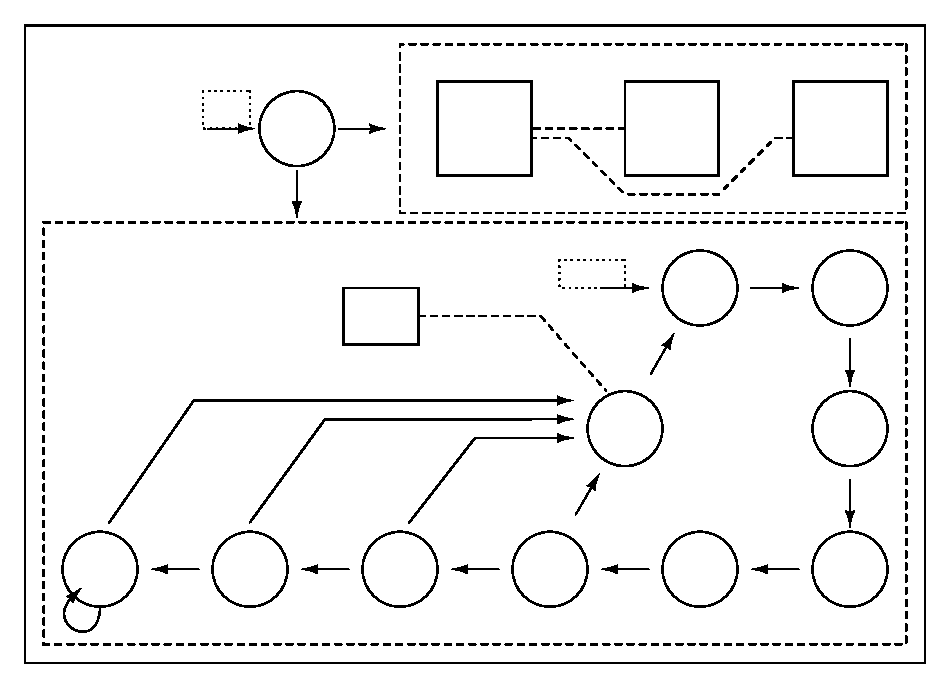
\includegraphics[scale=1.33333]{../media/hbussm.ps}\\
   % translate x=1600 y=896 scale 0.28
   \putbox{2.24in}{4.91in}{0.72}{Endpoint}%
   \putbox{2.24in}{4.74in}{0.72}{RX?}%
   \putbox{1.74in}{4.99in}{0.72}{Novo}%
   \putbox{1.74in}{4.91in}{0.72}{Byte}%
   \putbox{5.91in}{3.49in}{0.72}{RX}%
   \putbox{5.91in}{3.32in}{0.72}{SBID}%
   \putbox{7.24in}{3.49in}{0.72}{RX}%
   \putbox{7.24in}{3.32in}{0.72}{SDID}%
   \putbox{7.24in}{2.24in}{0.72}{RX}%
   \putbox{7.24in}{2.07in}{0.72}{SDID}%
   \putbox{7.24in}{0.99in}{0.72}{RX}%
   \putbox{7.24in}{0.82in}{0.72}{TBID}%
   \putbox{5.91in}{0.99in}{0.72}{RX}%
   \putbox{5.91in}{0.82in}{0.72}{TDID}%
   \putbox{4.57in}{0.99in}{0.72}{RX}%
   \putbox{4.57in}{0.82in}{0.72}{CMD}%
   \putbox{5.24in}{2.24in}{0.72}{RX}%
   \putbox{5.24in}{2.07in}{0.72}{STP}%
   \putbox{4.32in}{1.82in}{0.72}{BUSLOCK}%
   \putbox{4.16in}{1.66in}{0.72}{BUSUNLOCK}%
   \putbox{4.16in}{1.49in}{0.72}{SOFTRESET}%
   \putbox{4.41in}{1.32in}{0.72}{SEARCH}%
   \putbox{3.24in}{0.99in}{0.72}{RX}%
   \putbox{3.24in}{0.82in}{0.72}{ADDR}%
   \putbox{3.32in}{1.91in}{0.72}{QUERY}%
   \putbox{3.32in}{1.74in}{0.72}{GETCH}%
   \putbox{2.91in}{1.82in}{0.72}{CMD =}%
   \putbox{1.91in}{0.99in}{0.72}{RX}%
   \putbox{1.91in}{0.82in}{0.72}{PSZ}%
   \putbox{1.49in}{1.99in}{0.72}{CMD =}%
   \putbox{1.91in}{2.07in}{0.72}{STREAMW}%
   \putbox{1.91in}{1.91in}{0.72}{STREAMR}%
   \putbox{1.57in}{1.82in}{0.72}{ou}%
   \putbox{1.49in}{1.66in}{0.72}{PSZ = 0}%
   \putbox{0.57in}{0.99in}{0.72}{RX}%
   \putbox{0.57in}{0.82in}{0.72}{PRM}%
   \putbox{2.99in}{3.07in}{0.72}{Process}%
   \putbox{3.07in}{3.24in}{0.72}{Serial}%
   \putbox{3.91in}{3.24in}{0.72}{STP = 0xFF}%
   \putbox{2.57in}{4.24in}{0.72}{N}%
   \putbox{2.91in}{4.91in}{0.72}{S}%
   \putbox{3.91in}{4.91in}{0.72}{writeEP}%
   \putbox{3.99in}{4.74in}{0.72}{Byte}%
   \putbox{4.91in}{4.91in}{0.72}{FIM}%
   \putbox{5.57in}{4.91in}{0.72}{BUS}%
   \putbox{5.57in}{4.74in}{0.72}{UNLOCK}%
   \putbox{7.07in}{4.91in}{0.72}{EPwrite}%
   \putbox{7.07in}{4.74in}{0.72}{End}%
   \putbox{4.91in}{3.49in}{0.72}{RESET}%
   \putbox{0.16in}{5.57in}{0.72}{SERIAL\_RXBYTE}%
   \putbox{0.32in}{2.07in}{0.72}{RX CONT = PSZ}%
   } % close 'parbox'
   } % close 'scalebox'
   \vspace{-\baselineskip} % this is not necessary, but looks better
\end{center}

\caption{Máquina de estados de recepção HBUS}
\label{fig:hbussm}
\end{figure}

\subsection{A função SERIAL\_PROCESS()}

Esta função analisa o conteúdo do buffer local após a recepção com sucesso de um pacote. Note que são analisados todos os pacotes recebidos, independente se o destinatário é o dispositivo em questão ou não. Isto é necessário para que sejam detectados os eventos de travamento do barramento e endereçamento de dispositivos da maneira correta, atualizando a máquina de estados local.

Para resumir, é suficiente afirmar que esta função verifica os estados atuais do dispositivo: se o mesmo está ou não endereçado e se o barramento está travado para si próprio ou para outros dispositivos ou ainda livre e atua segundo o conjunto de informações.

Um fluxograma completo é complicado e redundante por demais, devido a quantidade de informação já discutida no documento até o momento. A figura a seguir limita-se a mostrar uma visão simplificada do que acontece quando o dispositivo não está endereçado.

\begin{figure}[H]
\centering
% XCircuit output "serialprocess.tex" for LaTeX input from serialprocess.ps
\def\putbox#1#2#3#4{\makebox[0in][l]{\makebox[#1][l]{}\raisebox{\baselineskip}[0in][0in]{\raisebox{#2}[0in][0in]{\scalebox{#3}{#4}}}}}
\def\rightbox#1{\makebox[0in][r]{#1}}
\def\centbox#1{\makebox[0in]{#1}}
\def\topbox#1{\raisebox{-0.60\baselineskip}[0in][0in]{#1}}
\def\midbox#1{\raisebox{-0.20\baselineskip}[0in][0in]{#1}}
\begin{center}
   \scalebox{0.75}{
   \normalsize
   \parbox{7.41667in}{
   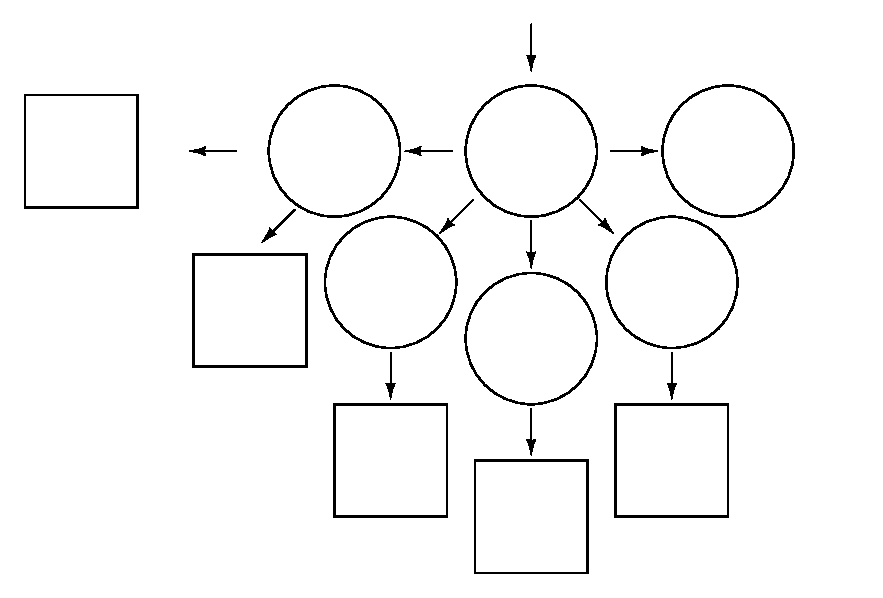
\includegraphics[scale=1.33333]{serialprocess.ps}\\
   % translate x=1472 y=928 scale 0.28
   \putbox{7.49in}{3.41in}{1.20}{}%
   \putbox{4.57in}{3.91in}{0.60}{\centbox{\midbox{DISP}}}%
   \putbox{4.57in}{3.74in}{0.60}{\centbox{\midbox{ENDERECADO?}}}%
   \putbox{4.66in}{3.07in}{0.60}{\centbox{\midbox{N}}}%
   \putbox{4.57in}{2.16in}{0.60}{\centbox{\midbox{CMD = BUSLOCK?}}}%
   \putbox{5.82in}{2.66in}{0.60}{\centbox{\midbox{CMD = BUSUNLOCK?}}}%
   \putbox{5.16in}{3.32in}{0.60}{\centbox{\midbox{N}}}%
   \putbox{4.66in}{1.41in}{0.60}{\centbox{\midbox{S}}}%
   \putbox{4.57in}{0.74in}{0.60}{\centbox{\midbox{BUS STATE = }}}%
   \putbox{4.57in}{0.57in}{0.60}{\centbox{\midbox{BUS LOCKED }}}%
   \putbox{4.57in}{0.41in}{0.60}{\centbox{\midbox{(OUTRO DISP)}}}%
   \putbox{6.32in}{0.99in}{0.60}{\centbox{\midbox{}}}%
   \putbox{5.91in}{1.91in}{0.60}{\centbox{\midbox{S}}}%
   \putbox{5.82in}{1.24in}{0.60}{\centbox{\midbox{BUS STATE = }}}%
   \putbox{5.82in}{0.99in}{0.60}{\centbox{\midbox{BUS FREE }}}%
   \putbox{3.32in}{2.66in}{0.60}{\centbox{\midbox{CMD = SOFTRESET?}}}%
   \putbox{3.99in}{3.24in}{0.60}{\centbox{\midbox{N}}}%
   \putbox{3.32in}{1.07in}{0.60}{\centbox{\midbox{RESET}}}%
   \putbox{3.41in}{1.91in}{0.60}{\centbox{\midbox{S}}}%
   \putbox{3.74in}{3.91in}{0.60}{\centbox{\midbox{N}}}%
   \putbox{2.82in}{3.82in}{0.60}{\centbox{\midbox{CMD = SEARCH?}}}%
   \putbox{1.82in}{3.32in}{0.60}{\centbox{\midbox{TDID = BROADCAST}}}%
   \putbox{2.07in}{2.57in}{0.60}{\centbox{\midbox{INICIA}}}%
   \putbox{2.07in}{2.32in}{0.60}{\centbox{\midbox{ENDERECAMENTO}}}%
   \putbox{1.74in}{3.16in}{0.60}{\centbox{\midbox{DISP S/ ENDERECO}}}%
   \putbox{1.74in}{4.16in}{0.60}{\centbox{\midbox{TDID = BROADCAST}}}%
   \putbox{1.74in}{3.99in}{0.60}{\centbox{\midbox{DISP ENDERECANDO}}}%
   \putbox{0.57in}{3.99in}{0.60}{\centbox{\midbox{FIM}}}%
   \putbox{0.57in}{3.74in}{0.60}{\centbox{\midbox{ENDERECAMENTO}}}%
   \putbox{5.41in}{3.91in}{0.60}{\centbox{\midbox{S}}}%
   \putbox{6.07in}{3.91in}{0.60}{\centbox{\midbox{}}}%
   \putbox{6.32in}{3.91in}{0.60}{\centbox{\midbox{PROCESSA}}}%
   \putbox{6.32in}{3.74in}{0.60}{\centbox{\midbox{BUFFER}}}%
   } % close 'parbox'
   } % close 'scalebox'
   \vspace{-\baselineskip} % this is not necessary, but looks better
\end{center}

\caption{A função SERIAL\_PROCESS() abreviada}
\end{figure}

\subsection{O envio de dados}

O envio de dados, como já discutido exaustivamente, não ocorre de forma espontânea, a não ser em caso de interrupção do dispositivo.

Logo, todos os envios de dados são dependentes dos estados do sistema. A maioria dos envios são realizados a partir da função SERIAL\_PROCESS(), que deve enviar vários dados em respostas a comandos emitidos pelo mestre.

Na revisão atual do barramento HBUS, o envio de dados é realizado manualmente colocando-se nas estruturas de dados as informações necessárias: tamanho em bytes do envio, endereço alvo e conteúdo da mensagem. Após isso, a variável de estado dos envios é colocada num estado que indica transmissão pendente. A função SERIAL\_CYCLE() verifica as pendências e se encarrega de realizar o envio. As estruturas de dados presentes relacionadas ao envio de dados:

\begin{itemize}

\item S\_TX\_SIZE : tamanho do envio em bytes
\item S\_TX\_NEXT : ponteiro para bytes a serem enviados
\item S\_TX\_NEXT\_ADDR : endereço do dispositivo alvo da transmissão
\item S\_TX\_STATE : estado da máquina de estados de envio (deve ser colocado em TX\_WAIT para iniciar um envio)

\end{itemize}

\subsection{A função SERIAL\_PROCESS\_TX()}

Esta função empacota um envio pendente, formatando-o ao padrão HBUS e realizando o envio através da UART do dispositivo.

\section{Segurança}

A partir da especificação versão 1.1 é adicionada o conceito opcional de privacidade de objetos e de autenticação do mestre.

Estas funcionalidades são opcionais ao dispositivo e incluem etapas adicionais no processamento dos comandos trafegados no barramento, incluindo a adição de mais dados no pacote, conforme o necessário.

Estes procedimentos são discutidos em maior detalhe num capítulo dedicado. No entanto, estão inseridos no escopo do protocolo de comunicação HBUS.
